\documentclass{report}

% Language setting
\usepackage[main=portuguese, english]{babel}
\usepackage{csquotes}

% Set page size and margins
\usepackage[a4paper,top=2cm,bottom=2cm,left=3cm,right=3cm,marginparwidth=1.5cm]{geometry}

% Useful packages
\usepackage{ulem}
\usepackage{parskip}
\usepackage{indentfirst}
\usepackage{setspace}
\usepackage{amsmath}
\usepackage{array}

\usepackage{graphicx}
\usepackage{xcolor}
\usepackage{colortbl}
\usepackage{subfigure}
\usepackage{titlesec}
\usepackage[colorlinks=false, allbordercolors={0 0 0}, pdfborderstyle={/S/U/W 0.25}]{hyperref}
\usepackage[hypcap=true]{caption}
\usepackage{enumitem}
\usepackage{soul}

\usepackage[
  backend=biber,
  style=apa,]{biblatex}
\addbibresource{reference.bib}

% Set section numbering from 1.1
\renewcommand{\thesection}{\arabic{section}.1}

\let\oldsection\section
\renewcommand\section{\clearpage\oldsection}

% Change section formatting
\titleformat{\section}
  {\fontsize{12}{15}\selectfont\bfseries}{\thesection}{1em}{}

% Configure indentations
\setlength{\parindent}{1.5cm}

\begin{document}

    \begin{titlepage}
        \centering
        
        \LARGE {Universidade Federal do Rio Grande do Sul \\ Instituto de Informática}
    
        \begin{figure}[h!]
        \centering
        \subfigure
        {
\includegraphics[width=0.35\linewidth]{images/logos/UFRGS.png}}
        \hspace{1cm}
        \subfigure
        {
\includegraphics[width=0.35\linewidth]{images/logos/INF.png}}
        \end{figure}
    
        \LARGE {INF01017 \\ Aprendizado de Máquina}
        
        \vfill
        {\noindent\hrulefill \\
        \bfseries \Huge{Atividade Prática 06} \\ \LARGE{Descrição dos Dados e Análise de Necessidades de Pré-processamento} \\
        \noindent\hrulefill}
        
        \vfill
        {\LARGE Luís Filipe Martini Gastmann (00276150) \\ Pedro Lubaszewski Lima (00341810) \\ Vinícius Boff Alves (00335551) \\~\\ Turma U}
    
        \vfill
        {\LARGE 9 de novembro de 2024}
        
    \end{titlepage}

        \renewcommand{\contentsname}{Sumário}
        \tableofcontents
        \clearpage
        \addtocontents{toc}{\protect\thispagestyle{empty}}

\section{Definição do Problema e Coleta de Dados}

O objetivo deste trabalho é prever o consumo médio de combustível de um carro através de algumas das suas características e origens de fabricação.
Alguns atributos das instâncias são a marca, a quantidade de cilíndros, o porte do veículo etc.

O conjunto de dados utilizado para desenvolver este trabalho foi obtido da seguinte página do Kaggle:
\href{https://www.kaggle.com/datasets/arslaan5/explore-car-performance-fuel-efficiency-data}{Explore Car Performance: Fuel Efficiency Data}.
Essa tarefa contará com diversas técnicas de preparação dos dados para posteriormente iniciar a seleção e
avaliação de modelos para essa tarefa.

\section{Análise Exploratória e Pré-processamento dos Dados}

Este \textit{dataset} possui 550 instâncias, com 11 atributos preditores e 1 atributo alvo. Esse último torna a tarefa dos modelos em regressão,
visto que o objetivo aqui é prever o consumo médio de combustível de carros. No conjunto de dados, esse atributo predito se chama \textit{combination mpg}.

Dos atributos preditores, observa-se que há 5 atributos numéricos (\textit{city mpg}, \textit{cylinders}, \textit{displacement}, \textit{highway mpg} e \textit{year}).
Além deles, os 6 atributos restantes são categóricos: \textit{class}, \textit{drive}, \textit{fuel type}, \textit{make}, \textit{model} e \textit{transmission}.
Com essa observação, já é previsto que será necessário fazer a codificação dos atributos categóricos e a normalização dos atributos numéricos. Para converter os atributos
categóricos em númericos, como são todos categoriais sem ordem estabelecida, será utilizada a codificação \textit{One-hot Encoding}. É claro que isso aumenta a dimensionalidade
do problema. Por conta disso, ainda será avaliado se serão necessárias medidas, como PCA, para reduzir a quantidade de atributos. Além disso, antes dessas conversões, o grupo
decidiu abandonar os atributos de \textit{city mpg} e \textit{highway mpg} por facilitarem demais o trabalho do preditor, visto que o atributo alvo, \textit{combination mpg},
pode ser calculado diretamente com esses dois atributos, algo que tornaria o modelo menos relevante. Se não for possível atingir uma métrica de qualidade satisfatória, alguma
dessas características pode ser reintroduzida no conjunto de dados. Portanto, o conjunto de dados acabou com 3 atributos numéricos normalizados e 6 atributos categóricos codificados.

Em relação a outras características das \textit{features} do problema, criou-se alguns gráficos para analisar correlações e distribuições dos dados. A seguir, o histograma
do atributo alvo pelo número de veículos:

\begin{figure}[h!]
  \centering
  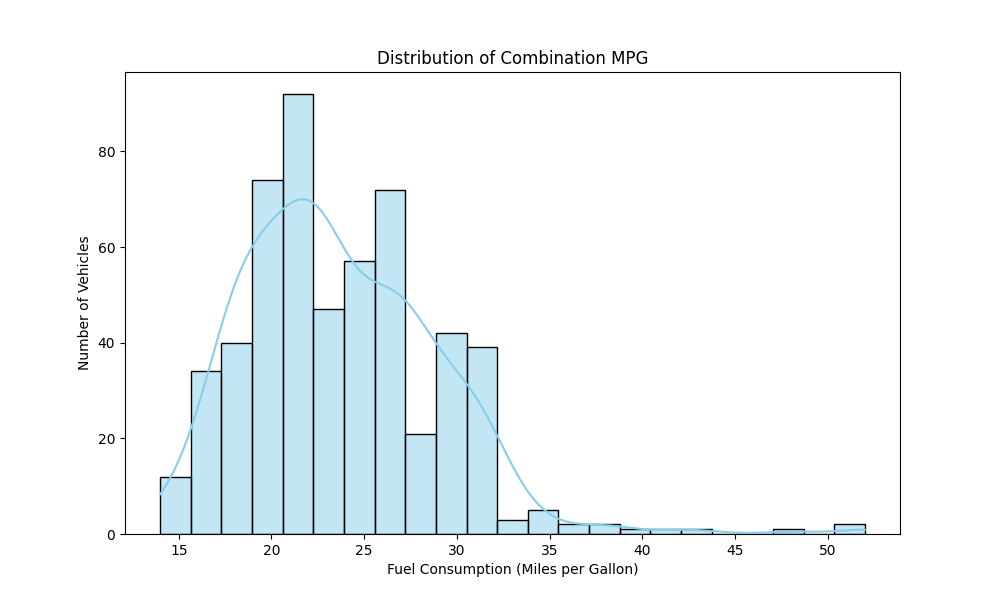
\includegraphics[width=\linewidth]{images/plots/combination_dist.png}
  \caption{\label{img:combination_dist} Histograma de Consumo Médio}
\end{figure}

Nesse gráfico, percebe-se que a maioria dos modelos tem consumo médio de combustível entre 20 e 30 mpg. Portanto, isso pode ser útil caso o grupo necessite realizar a remoção de \textit{outliers}
e também é problemático pois não há muitas instâncias com consumo acima de 35 mpg, tornando os modelos mais fracos nas predições com essa grandeza de consumo.

\clearpage
\begin{figure}[h!]
  \centering
  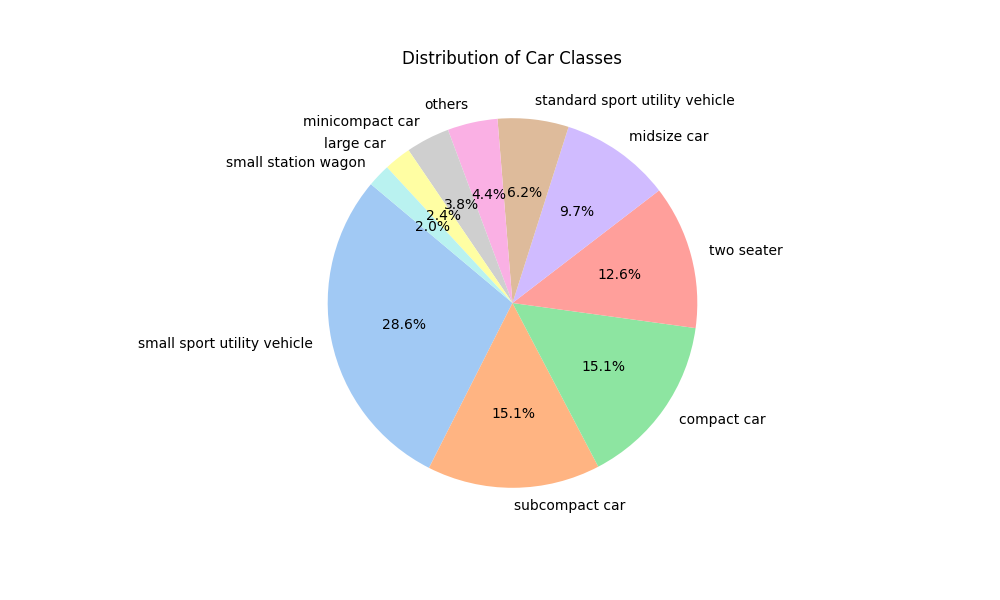
\includegraphics[width=\linewidth]{images/plots/classes_dist.png}
  \caption{\label{img:classes_dist} Distribuição de Classes de Veículos}
\end{figure}

Há diversas classes de veículos diferentes, com as mais diversas proporções. Por conta disso, adotar-se-á a política de agrupar essas classes e outros atributos
categoriais em uma classe chamada \textit{others} quando a quantidade de instâncias dela no conjunto de treinamento for insignificante para melhorar a generalização do modelo.

\begin{figure}[h!]
  \centering
  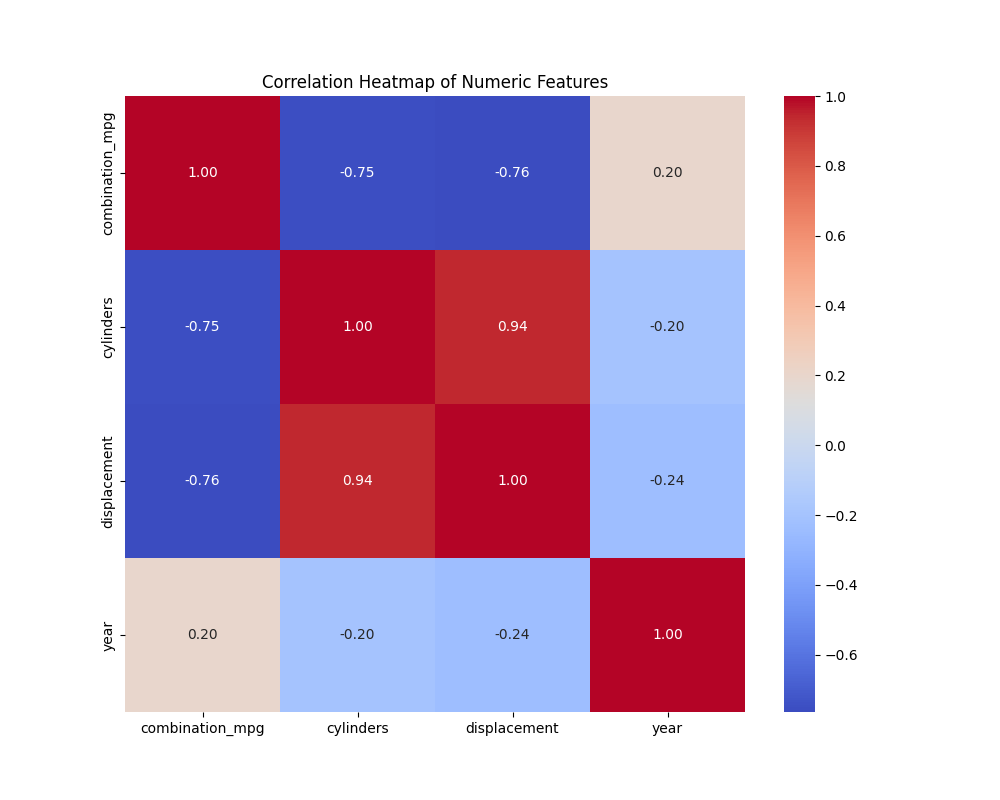
\includegraphics[width=\linewidth]{images/plots/num_heatmap.png}
  \caption{\label{img:num_heatmat} \textit{Heatmap} de Correlações entre Atributos Numéricos}
\end{figure}

No diagrama acima, são observadas as correlações dos atributos numéricos e do atributo alvo. Esse mapa foi feito através da Correlação de Pearson de cada um dos atributos.
Nele, é perceptível que bem possivelmente possa ser removido o atributo \textit{cylinders} ou (exclusivo) o atributo \textit{displacement}, visto que eles apresentam alto
índice de correlação, tornando a utilização dos dois redundante para os modelos.

Um outro problema encontrado consiste na possibilidade de não ser visto algum modelo de carro (\textit{model}) no treinamento. 
Isso pode acontecer pois há uma quantidade muito grande de modelos diferentes, alguns com poucas instâncias.
Para solucionar esse problema, ``forçou-se" a haver pelo menos uma instância de cada modelo de veículo no conjunto de treinamento.

\clearpage
%\printbibliography
\thispagestyle{empty}

\end{document}